\nsecbegin{Softwareverbreitung unter Linux}
%Autor: Tore Arndt

	\begin{itemize}
	\item Beschreibung
	
	
	Nach einiger Recherche bin ich im Internet auf eine vielversprechende Möglichkeit gestoßen, welche eine releativ einfache und weitrechende Lösung des Problems der Verbreitung von Software auf verschiedensten Linux-Distributionen zu bieten scheint.
	\textbf{Open Build Service} wurden von openSUSE für genau diesen Zweck entworfen.
	
	\item Was bietet Open Build Service?
	
	Open Build Service bietet die Möglichkeit ein Projekt automatisch für die meisten bekanntesten Linux Distributionen zur Verfügung zu stellen. Das Projekt wird über die Web UI hochgeladen und die zu unterstützenden Distributionen ausgewählt. OBS erstellt dann automatisch die nötigen Dependencies für alle ausgewählten Linux Distributionen und passt das Projekt automatisch an. Für alle Distributionen wird ein Download Link erstellt, über welchen die Nutzer die passende Version herunterladen können.
	
	\item Installation?
	
	Der Open Build Service (\textbf{OBS}) bietet eine online Plattform,
	allerdings muss ein Account unter \url{https://build.opensuse.org/} erstellt werden. \\
	Des weiteren erfordert die Nutzung des OBS auch noch die Installation des Command Line Interfaces (osc) dieses kann von openSUSE's GitHub Reposetory gecloned werden (\url{https://github.com/openSUSE/osc})\footnote{Um osc nutzen zu können wird zudem noch \textbf{python-xml} benötigt}.
	
	\item Wie funktioniert OBS?
	
	Die folgende Grafik zeigt anschaulich, wie der Open Build Service aufgebaut ist und wie Nutzer über die OBS API zugriff auf die verschiedenen Projektversionen erhalten.\\
	
	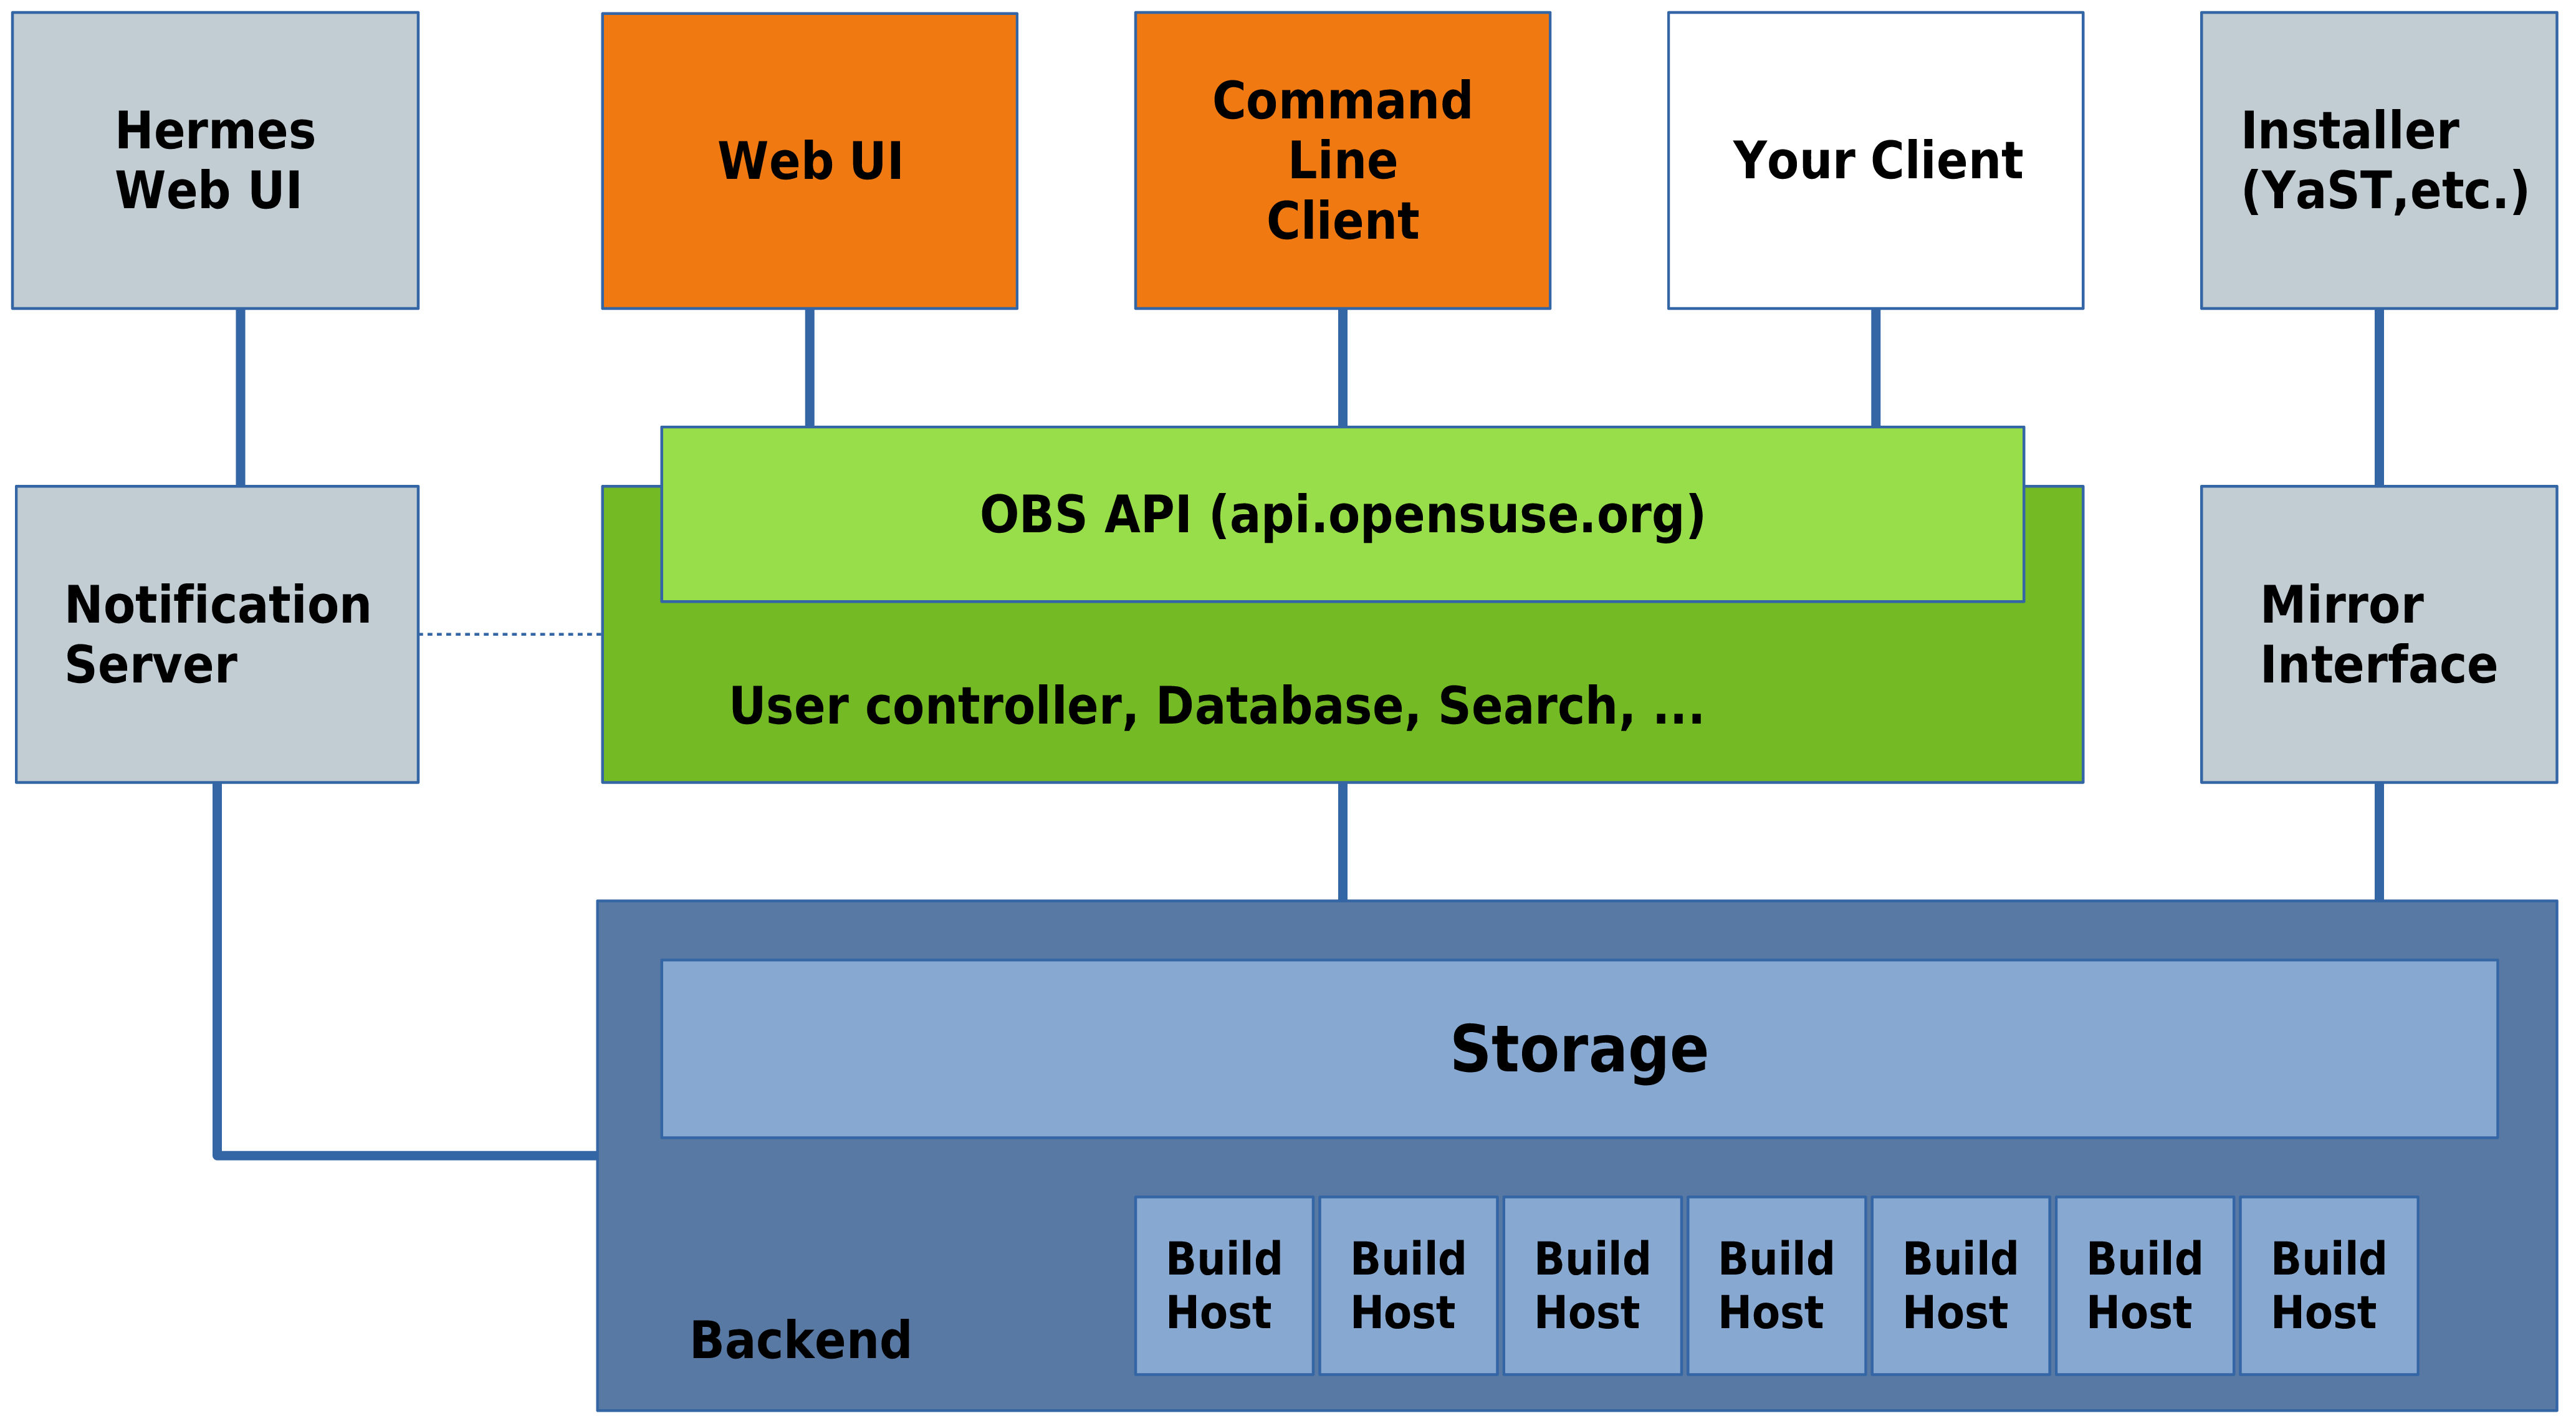
\includegraphics[width=\textwidth]{Bilder/obs-concept.jpg}\\
	
	\item Fazit
	
	OBS füllt zwar nicht genau die Anforderungen aus, da nicht eine Version für verschiedene Linux Distributionen erstellt wird, allerdings bietet er eine relativ gute Alternative, da die verschiedenen Versionen hier automatisch erstellt werden. Es sind allerdings einige Sachen als Vorraussetzung zu erfüllen und daher muss abgewogen werden, ob sich der Aufwand zu dem jetzigen Zeitpunkt lohnt.
	
	\item Extra
	
	Wärend meiner Recherche bin ich zudem auf ein interessantes Tool gestoßen, welches sich sehr gut als Ergänzung zum OBS einsetzen lässt.
	Das openQA, welches ebenso von openSUSE entwickelt wurde, bietet die Möglichkeit Programme auf deren Kompatibilität mit verschiedensten Betriebssystemen zu teste. \\
	Somit könnte man die mit OBS erstellten Versionen für verschiedene Linux Distributionen gleich auf deren Funktionalität testen. \\ (\url{open.qa})
	
	\item Quellen für weitere Informationen
	\begin{itemize}
		\item \url{https://www.ibm.com/developerworks/community/blogs/fe313521-2e95-46f2-817d-44a4f27eba32/entry/how_to_build_an_application_for_multiple_linux_distributions_from_a_single_source?lang=en}
		\item \url{https://openbuildservice.org/help/manuals/obs-beginners-guide/#co.obsbg.uc.basicprj.metadata}
		\item \url{https://openbuildservice.org/help/}
		\item \url{https://en.opensuse.org/openSUSE:Build_Service_Tutorial}
	\end{itemize}
	
	
	\end{itemize}

\nsecend


